\documentclass[a4paper,11pt]{article}
\author{Mathias Beke - 20120536\\ Jakob Struye - 20120612 \\ Robin Verachtert - 20121405}
\title{Codetheorie: \\Ontcijferopdracht}
\date{3 mei 2015}
\usepackage{hyperref}
\usepackage{listings}
\usepackage{seqsplit}
\usepackage{graphicx}
\usepackage[toc,page]{appendix}
\setcounter{section}{-1}


\begin{document}
\maketitle 
\tableofcontents
\pagebreak

\section{Inleiding}
Dit is het verslag van de resultaten van de ontcijferopdracht voor het vak codetheorie. Voor elk van de vijf opdrachten slaagden we erin de versleutelde boodschap volledig te ontcijferen. Bij de laatste opdracht vonden we alleen de titels van boeken gebruikt om sleutels te genereren niet. Voor elke opdracht volgen een tweetal pagina's over hoe we de opdracht aangepakt hebben, waar we eventueel moeilijkheden mee hadden en hoe we uiteindelijk het resultaat vonden. Daarna volgen nog twee appendices. Eerst hebben we een oplijsting van alle ontcijferde teskten en gebruikte sleutels, codewoorden en instellingen. We geven altijd de ontcijferde teksten zonder opmaak (spaties, kleine letters, leestekens), maar geven in de verslagen telkens een link naar een online versie met goede opmaak. In de tweede appendix staat beschreven hoe de code uitgevoerd kan worden. Hiermee is het mogelijk om onze resultaten te reconstrueren.


\section{Vigenere}
\subsection{Opdracht}
De eerste ciphertext was versleuteld met een Vigen\`ere cipher gevolgd door een enkele kolomtranspositie. Bij het ontcijferen moesten we dus eerst de kolomtranspositie ongedaan maken om een ciphertekst te bekomen die enkel met Vigen\`ere versleuteld was. 

\subsection{Ongedaan maken van de kolomtranspositie}
We zochten een manier om snel te checken of een ciphertekst met Vigen\`ere versleuteld was, zodat we de kolomtranspositie konden bruteforcen in een haalbare tijd. Hiervoor vonden we de "index of coincidence" (IC). Deze wordt als volgt berekend: $IC = \frac{\sum_{i=1}^{c}n_i(n_i -1)}{N(N-1)/c}$ met $n_i$ de frequenties van de $c$ verschillende letters in een tekst lengte $N$. In essentie is dit een frequentietabel samengevat in 1 waarde. Hoe groter de IC, hoe groter de kans dat twee willekeurig gekozen letters in een plaintext dezelfde zijn, met IC = 1 voor een random tekst waarbij elke letter evenveel voorkomt. Voor een Engelse tekst ligt de IC rond de 1.73. Merk op dat bij deze waarde geen rekening gehouden wordt met welke frequentie bij welke letter hoort. Dit betekent dat een plaintext na een monoalfabetische substitutie zijn IC behoudt. Bij een Vigen\`ere ciphertekst met sleutellengte n wordt op elke letter dezelfde monoalfabetische substitutie toegepast als op elke letter er op $kn$ posities vandaan ($k$ geheel). Als we een sleutellengte gokken, kunnen we de tekst verdelen in verzamelingen letters die met dezelfde substitutie versleuteld zouden zijn. Indien de gegokte lengte correct is, moet (indien de ciphertekst lang genoeg was) elke verzameling een redelijk hoge IC hebben, en moeten deze waarden redelijk dicht bij elkaar liggen. Indien de gegokte lengte fout is, zijn de letters in een verzameling niet met dezelfde monoalfabetische substitutie versleuteld (tenzij de gegokte lengte een veelvoud van de correcte is) en lijkt dit eerder een willekeurige verzameling letters, wat een IC dichter bij 1 zal opleveren. \\
Voor onze ciphertekst konden we dus alle mogelijke kolomtransposities ongedaan maken tot een bepaald aantal kolommen om dan te controleren of een mogelijke Vigen\`ere sleutellengte een hoge IC opleverde. Voor een ciphertext waarop een enkele kolomtranspositie toegepast is met $k \in [1,n]$ kolommen, zijn $\sum_{k=1}^{n}k!$ transposities mogelijk. Dit wordt al snel onmogelijk om in een haalbare tijd uit te rekenen, maar gelukkig is het aantal kolommen doorgaans klein. \\
Het ongedaan maken van de transposities gebeurt voor elke mogelijke permutatie van k kolommen als volgt: de ciphertekst lengte $l$ bestaat uit opeenvolgend de letters uit kolommen 1 t.e.m. $k$. In elke kolom komen minstens $\lfloor\frac{l}{k}\rfloor$ voor. In de eerste $l\%k$ kolommen (in de volgorde bepaald door het codewoord voor de kolomtranspositie = gepermuteerde kolommen) komt nog 1 extra letter voor, zodat alle kolommen samen uiteindelijk $l$ letters bevatten. We kunnen de kolommen makkelijk opvullen door gewoon de ciphertekst te overlopen en 1 voor 1 de kolommen op te vullen. Daarna overlopen we de kolommen round-robin in gepermuteerde volgorde en halen we telkens de eerstvolgende letter uit de kolom. In deze volgorde vormen de letters de ciphertekst voor de kolomtranspositie. Op elk van deze cipherteksten voeren we dan, voor elke mogelijke sleutellengte $l$ tot een bepaalde waarde, de volgende Vigen\`eretest uit: we verdelen de ciphertekst in $l$ groepen door de letters 1 voor 1 round-robin over de groepen te verdelen. Elk van deze groepen zou dan door dezelfde monoalfabetische substitutie versleuteld zijn. We berekenen de IC van elke groep en dan het gemiddelde ervan. Indien dit gemiddelde boven een vooraf ingestelde waarde komt, is dit waarschijnlijk de correctie sleutellengte (of een veelvoud ervan). \\ \\ Bij het toepassen van dit principe bij de gegeven ciphertekst, moesten we eerst wat spelen met de variabelen (maximale keylengtes voor Vigen\`ere en kolomtranspositie en minimale IC), maar uiteindelijk vonden we (met een runtime van slechts een viertal seconden) zes kolomtransposities van zes kolommen waarbij Vigen\`ere met sleutellengte 8 een IC van ongeveer 2.15 opleverde. Na vergelijken met wat andere zelf berekende IC's van Nederlandstalige teksten, waren we hier al redelijk zeker dat deze plaintekst Nederlands was. 

\subsection{Vigenere oplossen}
Daarna berekenden we bij elk van de zes mogelijke transposities voor elk van de 8 groepen letters de meest voorkomende letter. Aannemend dat dit de E was (in het Nederlands erg waarschijnlijk) konden we meteen de monoalfabetische substitutie ongedaan maken op elke groep. Door de volgorde van de letters te reconstrueren, bekwamen we bij een van de zes transposities de volgende plaintekst, een fragment uit "Erik of het Klein Insectenboek" door Godfried Bomans.




\section{Playfair}
\subsection{De opdracht}
De tweede ciphertext was versleuteld met Playfair. We moesten dus de key zien te vinden waarmee een matrix was opgesteld om digrammen te versleutelen. We hadden op dit punt al een Nederlandse en een Franse tekst ontcijferd, dus we gingen ervanuit dat dit Engels was. 
Het oplossen van Playfair bleek moeilijker als ADFGVX en Vigenere, na 3 gefaalde pogingen is het ons uiteindelijk gelukt.

\subsection{Poging 1: frequentieanalyse}
Onze eerste poging bestond uit een frequentieanalyse van de digrammen. We vergeleken die waarden met gekende waarden voor digrammen in het Engels die we zelf hadden berekend aan de hand van enkele Engelse teksten. Na veel puzzelwerk raakten we echter niet erg ver. Er zijn 600 digrammen in Playfair (hoewel ze niet allemaal in de ciphertext voorkwamen) en door dicht bij elkaar gelegen frequenties was het bijna onmogelijk ze juist te kiezen. We bekeken ook de frequenties van opeenvolgende digrammen samen en we hielden rekening met frequente digrammen waarvan ook het omgekeerde frequent was, maar raakten ook hiermee niet verder.

\subsection{Poging 2: slimme frequentie analyse}
Aangezien we door gewoon naar de frequenties te kijken toch 2 digrammen vrij zeker wisten ("OS" $\leftrightarrow$ "th", "OB" $\leftrightarrow$ "he"), probeerden we om gebruik te maken van de structuur van het Playfairvierkant\footnote{\url{http://www.umich.edu/~umich/fm-34-40-2/ch7.pdf}}. Dit werkte echter ook niet, omdat we geen van de andere digrammen echt zeker wisten, en diegenen die we dachten juist te gokken niet in het vierkant bleken te passen. We probeerden de ciphertext te bruteforcen met keys waarbij deze reeds gevonden digrammen klopten, maar vonden ook zo het antwoord niet.
 
\subsection{Poging 3: Hill Climb Algoritme}
Daarna gooiden we het over een andere boeg en gingen we op zoek naar een algoritme om de ciphertext volledig geautomatiseerd te kraken. Eerst maakten we een implementatie van een hill climb algoritme. We startten door uit een startset van mogelijke keys (in ons geval 100 random gekozen keys) de besten op basis van Index of Coincedence\footnote{\url{http://practicalcryptography.com/cryptanalysis/text-characterisation/index-coincidence/}}\footnote{\url{http://en.wikipedia.org/wiki/Index_of_coincidence}} te selecteren en deze te wijzigen. Die gewijzigde keys beschouwden we dan als nieuwe startset. Op een gegeven moment bereiken we een (lokaal) maximum, wat als resultaat gezien wordt. Doordat we bij het wijzigen telkens de best scorende keys uit heel wat opties selecteerden, werkte het algoritme redelijk traag of belandde het direct in een lokaal maximum.

\subsection{Poging 4: Churn Algoritme}
Daarna stootten we op het zogenaamde Churn algoritme \footnote{\url{http://www.cryptoden.com/index.php/algorithms/churn-algorithm/20-churn-algorithm}} \footnote{\url{http://s13.zetaboards.com/Crypto/topic/6781204/1/}}. Dit algoritme is gelijkaardig aan simulated annealing, alleen heel wat simpeler om te implementeren. \\ 
Elke plaintext krijgt een score toegewezen als volgt: voor elke mogelijke digram in het Engels werd de frequentie geanalyseerd. Hiervan werden telkens de log genomen om de invloed van erg grote waarden te beperken, en werden deze waarden herschaald naar 0-9. Nu is de score van de plaintext de som van de frequenties van elk van de $l-1$ digrams in de plaintext lengte $l$. Hoe hoger de score, hoe waarschijnlijker dat de tekst Engels is. In het algoritme starten we met een zogenaamde parent key (bv. gewoon het alfabet) waarmee we de ciphertext ontcijferen en een score toekennen. Daarna voeren we een kleine verandering (permutatie van letters, kolommen of rijen) door aan de parent key en noemen we het resultaat de child key. De plaintext voor de child key wordt ook ge\"evalueerd. Indien de child key beter scoorde, vervangt deze de parent key. Indien de parent key beter scoorde, wordt een willekeurig getal uit een array van 100 getallen gekozen. Indien het verschil tussen parent en child key scores minder was dan dit gekozen getal, vervangt de child key toch de parent key. Hierdoor kan het algoritme uit lokale maxima raken. Het algoritme blijft oneindig lopen en print de uitkomst van een iteratie enkel indien een nieuwe topscore bereikt is. Merk op dat de 100 getallen in de genoemde array zodanig gekozen zijn dat de kans dat child parent vervangt, gelijkaardig is aan die bij simulated annealing. Bij sommige runs van het algoritme vonden we al na een tweeduizendtal iteraties een tekst die heel erg op Engels leek. Het antwoord was niet helemaal correct gezien bij de score geen rekening gehouden werd met de meer voorkomende X bij Playfair. Het was wel dicht genoeg bij Engels dat we de laatste aanpassingen handmatig konden doorvoeren. We vonden als key "A brief history of time", met als plaintext het begin van "A Brief History of Time: From the Big Bang to Black Holes" door Stephen Hawking. \footnote{\url{http://www.fisica.net/relatividade/stephen_hawking_a_brief_history_of_time.pdf\#page=3}}. Merk op dat we de twee lijsten met waarden op \url{http://www.cryptoden.com/} vonden, maar de code verder helemaal zelf geschreven is en enkel gebaseerd is op de beschrijving van het algoritme.Het bijbehorende vierkant is hieronder afgebeeld.   \\
\subsection{Verbeteringen aan het algoritme}
Het algoritme in playfair.py is een licht aangepaste versie van wat we eerst gebruikten. Het geeft vaker snel een antwoord door rollbacks uit te voeren als een tijdje geen vooruitgang geboekt wordt, of zelfs helemaal opnieuw te beginnen. Ook is het scoren nu aangepast aan de X'en in Playfair waardoor exact de correcte plaintext wordt gevonden. De gevonden key matrix is niet altijd de matrix gegenereerd met "abriefhistoryoftime", maar wel altijd een correcte matrix. Gezien niet alle digrammen voorkomen, zijn meerdere correcte matrices mogelijk. \\
In de eerste twee lijntjes van het Churn algoritme wordt een vaste seed ingesteld. Deze levert al na 2406 iteraties het antwoord op. Om met een andere seed te proberen, moeten de eerste twee regels code verwijderd worden. Hierdoor kan het algoritme wel langer duren. De vari\"erende runtime is een gevolg van de niet-deterministische aard van het algoritme. Gezien de code niet concurrent is, is het aangewezen om het programma meerdere keren tegelijk te draaien om sneller tot een resultaat te komen.

\begin{figure} [h!]
\centering
\begin{tabular}{c|c|c|c|c}
A&B&R&I&E\\ \hline
F&H&S&T&O\\ \hline
Y&M&D&G&J\\ \hline
K&L&N&P&Q\\ \hline
U&V&W&X&Z\\
\end{tabular}
\caption{Playfairvierkant key "A brief history of time"}
\end{figure}


\documentclass[a4paper,11pt]{article}
\author{Robin Verachtert - s0121405}
\title{Cryptografie en Codetheorie: \\ADFGVX}
\date{10 march 2015}
\usepackage{hyperref}
\usepackage{listings}

\urldef{\googleSearch}\url{https://www.google.be/search?q=l%27annee+1966+fut+marquee+par+une+evenement&oq=l%27annee+1966+fut+marquee+par+une+evenement&aqs=chrome..69i57.1740j0j7&sourceid=chrome&es_sm=122&ie=UTF-8#q=l%27annee+1966+fut+marquee+par+un+evenement+bizarre} % define url in heading, because otherwise the % give problems


\begin{document}
%\maketitle 
%\tableofcontents
%\pagebreak
\section{ADFGVX}
\subsection{De kolomtranspositie}
Aangezien ADFGVX eindigt met een enkele kolomtranspositie, moesten we deze eerst ongedaan maken. Hiervoor gebruikten we hetzelfde systeem als beschreven bij Vigenère: voor alle mogelijke transposities tot een bepaald aantal kolommen werd de index of coincidence berekend, waarna die met de hoogte index gekozen werd. Merk op dat we hierbij de digrammen moesten gebruiken om de index te berekenen. Uiteindelijk vonden we 4 mogelijke kolomtransposities met 4 kolommen, met elk een even grote IC.

\subsection{Vinden van de taal.}
Door eerst een frequentieanalyse te doen op de 4 meest waarschijnlijke teksten, kregen we de onderstaande tabel.
\begin{center}
\begin{tabular}{|c|c|c|c|c|c|c|c|}
\hline
'FV'& 16.93 &
'AA'& 8.26 &
'DX'& 8.02 &
'AD'& 7.80\\ \hline
'XV'& 7.32 &
'VD'& 7.18 &
'AF'& 6.15 &
'FF'& 5.80\\ \hline
'GG'& 5.64 &
'DD'& 4.91 &
'XD'& 3.64 &
'XG'& 3.18\\ \hline
'FA'& 3.10 &
'DG'& 2.94 &
'VX'& 1.59 &
'DF'& 1.21\\ \hline
'VA'& 1.16 &
'VG'& 1.16 &
'GF'& 0.99 &
'GD'& 0.67\\ \hline
'AV'& 0.56 &
'GX'& 0.51 &
'FG'& 0.32 &
'XX'& 0.13\\ \hline
'AG'& 0.13 &
'VV'& 0.10 &
'FD'& 0.08 &
'XF'& 0.08\\ \hline
'FX'& 0.05 &
'XA'& 0.05 &
'DA'& 0.05 &
'VF'& 0.05\\ \hline
'DV'& 0.05 &
'AX'& 0.02 &
'GA'& 0.0 &
'GV'& 0.0\\ \hline
\end{tabular}

%\caption{ Tabel met de digram frequenties voor de tekst verkregen door de 4e kolom transpositie. De andere frequentie tabellen zijn bijna identiek, alleen zijn de digrammen anders.}
\end{center}

Om deze tabel te analyseren vergelijken we hem gewoon met gekende frequenties\footnote{\url{http://en.wikipedia.org/wiki/Letter_frequency}}. Dit kan omdat de digrammen in ADFGVX voor enkele characters staan. In ADFGVX kan men ook cijfers gebruiken. Deze staan niet in de frequentietabellen vermeld, maar dit is niet echt een probleem, aangezien deze waarschijnlijk een redelijk kleine frequentie hebben. Dit gaf ons wel een vervormde index of coincidence, waardoor we puur op deze waarde de taal niet konden bepalen. Het viel ons wel op dat het meest voorkomende digram, 'FV' bijna dubbel zo frequent was als het tweede. Van de waarschijnlijke talen voor deze tekst, zijn het Frans en Duits de enige met dit kenmerk. Aangezien de Enigma code in het Duits is, is het zeer waarschijnlijk dat deze tekst in het Frans is geschreven.

\subsection{Vinden van de bron tekst}

Voordat we begonnen met letters te vervangen hebben we eerst het aantal mogelijke teksten terug gebracht van 4 naar 2. We hebben dit gedaan door te kijken naar de digrammen die 2 maal op elkaar volgen. Bij twee van de vier mogelijke teksten kwam een opeenvolging van twee keer hetzelfde digram erg veel voor. Gezien dit in het Frans minder voorkomt, konden we deze teksten al elimineren.

Nu we nog 2 mogelijke teksten hadden, hebben we het werk opgesplitst onder Jakob en Robin, die elks een tekst probeerden te kraken.

Door eerst de meest frequente letters in te vullen (FV=e, DX=n, ... ) en daarna met trial en error de andere redelijk frequente characters in te vullen, verschenen er Franse woorden, of strings die erg leken op een Frans woord, hierdoor konden we ook de minder frequente letters invullen. Eens ongeveer de helft van de digrammen was vervangen door een character, konden we zinnen lezen en zo de andere characters aanvullen, eens we de eerste zin zeker wisten konden we Google aanspreken \footnote{\googleSearch} en vonden we dat het ging om het eerste hoofdstuk van \textit{"Vingt mille lieues sous les mers"} van Jules Vernes. 

Zoals reeds vermeld hadden we 2 teksten opgelost, beide gaven dezelfde tekst. Als we kijken naar de vierkanten die beiden gaven (Figure 2 en 3), zien we dat de ene de getransponeerde versie van de andere is. Dit betekent dat de digrammen voor de ene versie de omgekeerde zijn van de andere versie. Ene ene ciphertekst is dus gelijk aan de andere ciphertekst met elk digram omgedraaid, voor de kolomtranspositie. Gezien de kolomtranspositie met een even aantal kolommen gebeurde, kan door een verschillende kolomtranspositie toe te passen op beide teksten, dezelfde uiteindelijke ciphertekst bekomen worden.

\begin{figure}[h!]
   \begin{minipage}{0.45\textwidth}
		\begin{tabular}{c || c | c | c | c | c | c |}
		&A&D&F&G&V&X\\	\hline\hline
		A&a&5&c&?&q&w\\ \hline
		D&s&o&2&x&i&d\\ \hline
		F&r&g&l&b&0&1\\ \hline
		G&6&m&y&u&f&p\\ \hline
		V&h&3&e&?&z&t\\ \hline
		X&4&n&8&j&v&k\\ \hline
		\end{tabular}
		\caption{Vierkant van de 1e tekst }
    \end{minipage}
      \hspace{0.5cm}
   \begin{minipage}{0.45\textwidth}
		\begin{tabular}{c || c | c | c | c | c | c |}
		&A&D&F&G&V&X\\	\hline\hline
		A&a&s&r&6&h&4\\ \hline
		D&5&o&g&m&3&n\\ \hline
		F&c&2&i&y&e&8\\ \hline
		G&?&x&b&u&?&j\\ \hline
		V&q&l&0&f&z&v\\ \hline
		X&w&d&1&p&t&k\\ \hline
		\end{tabular}
		\caption{Vierkant van de 2e tekst }
    \end{minipage}
\end{figure}

\end{document}

\pagebreak %for style purposes
\documentclass[11pt, a4paper]{article}

\usepackage{seqsplit}
\usepackage{hyperref}
\usepackage{graphicx}



\begin{document}

De vierde ciphertekst was versleuteld met Enigma. Eerst implementeerden we een volledige Enigma machine. Daarna gingen we op zoek naar de gebruikte rotoren en hun beginstand. Er was een crib gegeven, dus we konden makkelijk een crib graph opstellen. Hiervoor stelden we manueel een .dot file om, waarmee we een visuele voorstelling genereerden. Deze is hieronder weegegeven. \\
\begin{center}
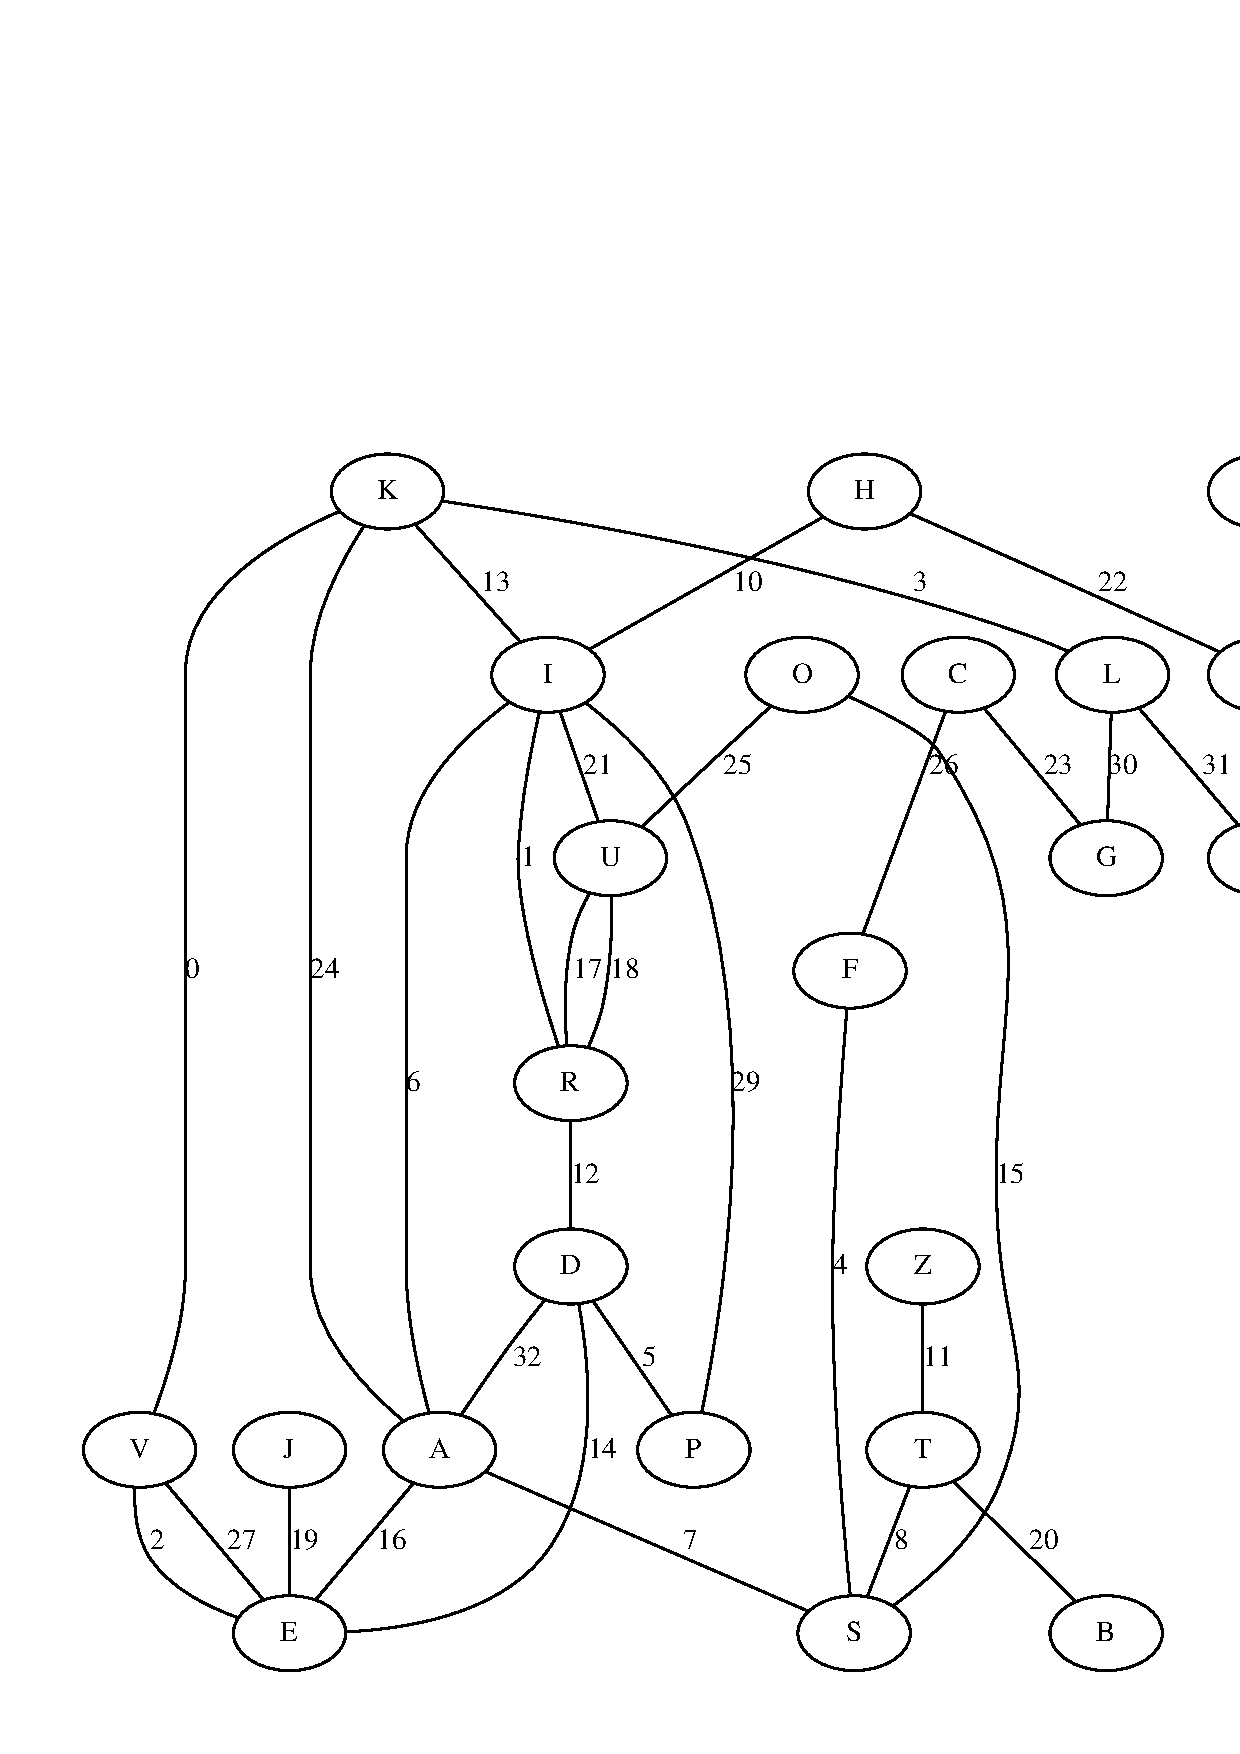
\includegraphics[scale=0.25]{graph.png}
\end{center}  
Aan de hand van de graph konden we op zoek naar gesloten paden. Door de lengte van de crib waren er heel wat mogelijkheden. We bepaalden voor de letter U 6 gesloten paden. We gingen dan, met elke mogelijke volgorde van rotoren, op zoek naar een k waarvoor een letter invariant bleef op elk van die paden. Hiervoor was een kleine modificatie aan onze ge\"implementeerde Engima machine voldoende. We vonden dat er hiervoor slechts \'e\'en optie was, namelijk rotorvolgorde 420 met als beginstand KSY. De invariante letter was hier de U, wat betekent dat de U door het plugboard niet aangepast wordt. We herhaalden deze test met de letters A, D en I, waarvoor we ook telkens 5 \`a 6 gesloten paden zochten. Hier vonden we ook telkens slechts 1 of 2 resultaten, waaronder altijd rotorvolgorde 420 met beginstand KSY. Dit was dus zeker het juiste antwoord. Uit deze resultaten vonden we ook dat het plugboard I en Y verwisselt, en de A en de D niet aanpast. Nu moesten we enkel nog op zoek naar de rest van het plugboard. Omdat we een behoorlijk grote crib hadden, waren er voor de meeste letters gesloten paden te vinden in de graph. We konden dus gewoon een versimpelde versie van de voorgaande code draaien voor elke letter met gesloten paden om het plugboard verder te bepalen. Hiervoor hoefden we de test enkel voor de correcte rotorvolgorde en beginstand draaien. De enige letters zonder gesloten paden waren B, J, Q, T, W, X, Y en Z waarbij Q, W en X helemaal niet in de graph voorkwamen, en we al wisten dat Y met I werd omgewisseld. We gingen dus enkel de mappings van de letters met gesloten paden zoeken. Hierdoor vonden we ook de mappings voor B, Q, W en Z omdat ze elk verwisseld werden met een letter die wel gesloten paden had. We hadden het plugboard dus op J, T en X na bepaald. Er waren nu echter maar 4 mogelijke plugboards over: ofwel werden twee van de drie letters met elkaar gewisseld ofwel werd geen enkele gewisseld. Door de ciphertekst met elk van de vier opties te decipheren, vonden we dat enkel die waarbij J, T en X niet werden aangepast de crib juist ontcijferde en dus juist was. Hiermee hadden we ook het plugboard volledig bepaald en konden we de tekst volledig ontcijferen. Het was een deel uit Die Blechtrommel van G\"unter Grass \footnote{\url{http://www.lawrenceglatz.com/germ3230/texte/grass1.htm}}.



Rotorvolgorde: 420 \\
Beginstand: KSY \\
Plugboard:  KEDCHGFYJBLWNZPSRQTUVMXIO \\
Verwisselingen in plugboard: B-K, C-E, F-H, I-Y, M-W, O-Z, Q-S \\
\seqsplit{VIELSPASSMITDIESERUEBUNGAUFENIGMAZUGEGEBENICHBININSASSEEINERHEILUNDPFLEGEANSTALTMEINPFLEGERBEOBACHTETMICHLASSTMICHKAUMAUSDEMAUGEDENNINDERTURISTEINGUCKLOCHUNDMEINESPFLEGERSAUGEISTVONJENEMBRAUNWELCHESMICHDENBLAUAUGIGENNICHTDURCHSCHAUENKANNMEINPFLEGERKANNALSOGARNICHTMEINFEINDSEINLIEBGEWONNENHABEICHIHNERZAHLEDEMGUCKERHINTERDERTURSOBALDERMEINZIMMERBETRITTBEGEBENHEITENAUSMEINEMLEBENDAMITERMICHTROTZDESIHNHINDERNDENGUCKLOCHESKENNENLERNTDERGUTESCHEINTMEINEERZAHLUNGENZUSCHATZENDENNSOBALDICHIHMETWASVORGELOGENHABEZEIGTERMIRUMSICHERKENNTLICHZUGEBENSEINNEUESTESKNOTENGEBILDEOBEREINKUNSTLERISTBLEIBEDAHINGESTELLTEINEAUSSTELLUNGSEINERKREATIONENWURDEJEDOCHVONDERPRESSEGUTAUFGENOMMENWERDENAUCHEINIGEKAUFERHERBEILOCKENERKNOTETORDINAREBINDFADENDIEERNACHDENBESUCHSSTUNDENINDENZIMMERNSEINERPATIENTENSAMMELTUNDENTWIRRTZUVIELSCHICHTIGVERKNORPELTENGESPENSTERNTAUCHTDIESEDANNINGIPSLASSTSIEERSTARRENUNDSPIESSTSIEMITSTRICKNADELNDIEAUFHOLZSOCKELCHENBEFESTIGTSINDOFTSPIELTERMITDEMGEDANKENSEINEWERKEFARBIGZUGESTALTENICHRATEDAVONABWEISEAUFMEINWEISSLACKIERTESMETALLBETTHINUNDBITTEIHNSICHDIESESVOLLKOMMENSTEBETTBUNTBEMALTVORZUSTELLENENTSETZTSCHLAGTERDANNSEINEPFLEGERHANDEUBERDEMKOPFZUSAMMENVERSUCHTINETWASZUSTARREMGESICHTALLENSCHRECKENGLEICHZEITIGAUSDRUCKZUGEBENUNDNIMMTABSTANDVONSEINENFARBIGENPLANENMEINWEISSLACKIERTESMETALLENESANSTALTSBETTISTALSOEINMASSSTABMIRISTESSOGARMEHRMEINBETTISTDASENDLICHERREICHTEZIELMEINTROSTISTESUNDKONNTEMEINGLAUBEWERDENWENNMIRDIEANSTALTSLEITUNGERLAUBTEEINIGEANDERUNGENVORZUNEHMENDASBETTGITTERMOCHTEICHERHOHENLASSENDAMITMIRNIEMANDMEHRZUNAHETRITTEINMALINDERWOCHEUNTERBRICHTEINBESUCHSTAGMEINEZWISCHENWEISSENMETALLSTABENGEFLOCHTENESTILLEDANNKOMMENSIEDIEMICHRETTENWOLLENDENENESSPASSMACHTMICHZULIEBENDIESICHINMIRSCHATZENACHTENUNDKENNENLERNENMOCHTENWIEBLINDNERVOSWIEUNERZOGENSIESINDKRATZENMITIHRENFINGERNAGELSCHERENANMEINEMWEISSLACKIERTENBETTGITTERKRITZELNMITIHRENKUGELSCHREIBERNUNDBLAUSTIFTENDEMLADELANGGEZOGENEUNANSTANDIGESTRICHMANNCHENMEINANWALTSTULPTJEDESMALSOBALDERMITSEINEMHALLODASZIMMERSPRENGTDENNYLONHUTUBERDENLINKENPFOSTENAMFUSSENDEMEINESBETTESSOLANGESEINBESUCHWAHRTUNDANWALTEWISSENVIELZUERZAHLENRAUBTERMIRDURCHDIESENGEWALTAKTDASGLEICHGEWICHTUNDDIEHEITERKEITNACHDEMMEINEBESUCHERIHREGESCHENKEAUFDEMWEISSENMITWACHSTUCHBEZOGENENTISCHCHENUNTERDEMANEMONENAQUARELLDEPONIERTHABENNACHDEMESIHNENGELUNGENISTMIRIHREGERADELAUFENDENODERGEPLANTENRETTUNGSVERSUCHEZUUNTERBREITENUNDMICHDENSIEUNERMUDLICHRETTENWOLLENVOMHOHENSTANDARDIHRERNACHSTENLIEBEZUUBERZEUGENFINDENSIEWIEDERSPASSANDEREIGENENEXISTENZUNDVERLASSENMICHDANNKOMMTMEINPFLEGERUMZULUFTENUNDDIEBINDFADENDERGESCHENKPACKUNGENEINZUSAMMELNOFTMALSFINDETERNACHDEMLUFTENNOCHZEITANMEINEMBETTSITZENDBINDFADENAUFDROSELNDSOLANGESTILLEZUVERBREITENBISICHDIESTILLEBRUNOUNDBRUNODIESTILLENENNEBRUNOMUNSTERBERGICHMEINEJETZTMEINENPFLEGERLASSEDASWORTSPIELHINTERMIRKAUFTEAUFMEINERECHNUNGFUNFHUNDERTBLATTSCHREIBPAPIERBRUNODERUNVERHEIRATETKINDERLOSISTUNDAUSDEMSAUERLANDSTAMMTWIRDSOLLTEDERVORRATNICHTREICHENDIEKLEINESCHREIBWARENHANDLUNGINDERAUCHKINDERSPIELZEUGVERKAUFTWIRDNOCHEINMALAUFSUCHENUNDMIRDENNOTWENDIGENUNLINIERTENPLATZFURMEINHOFFENTLICHGENAUESERINNERUNGSVERMOGENBESCHAFFENNIEMALSHATTEICHMEINEBESUCHERETWADENANWALTODERKLEPPUMDIESENDIENSTBITTENKONNENBESORGTEMIRVERORDNETELIEBEHATTEDENFREUNDENSICHERVERBOTENETWASSOGEFAHRLICHESWIEUNBESCHRIEBENESPAPIERMITZUBRINGENUNDMEINEMUNABLASSIGSILBENAUSSCHEIDENDENGEISTZUMGEBRAUCHFREIZUGEBENALSICHZUBRUNOSAGTEACHBRUNOWURDESTDUMIRFUNFHUNDERTBLATTUNSCHULDIGESPAPIERKAUFENANTWORTETEBRUNOZURZIMMERDECKEBLICKENDUNDSEINENZEIGEFINGEREINENVERGLEICHHERAUSFORDERNDINDIEGLEICHERICHTUNGSCHICKENDSIEMEINENWEISSESPAPIERHERROSKAR}

\end{document}

\section{Diffie-Hellman}
\subsection{De opdracht}
De opdracht rond Diffie-Hellman bestond uit twee delen: ten eerste het berekenen van de gezamenlijke sleutel en ten tweede het achterhalen van de titels waaruit de geheime sleutels gegenereerd werden.

\subsection{Gezamenlijke sleutel: eerste pogingen}
Het snelste algoritme dat we in de les zagen om dit te ontcijferen, is index calculus. We probeerden dit dus te implementeren. Dit bleek echter een redelijk ingewikkelde zaak. Er moeten heel wat keuzes gemaakt worden tijdens het algoritme (set van priemgetallen om mee te werken, ...) wat moeilijk in code te gieten is. Daarnaast moeten er heel wat priemontbindingen berekend worden. Relatief snelle algoritmes hiervoor zijn heel ingewikkeld en vielen voor ons niet te implementeren. Applicaties die snel priemontbindingen berekenen zoals Wolfram-Alpha, gebruiken hiervoor een combinatie van algoritmes tot \'e\'en ervan een resultaat vindt. Dit soort implementaties is voor ons uiteraard onhaalbaar. Index calculus bleek voor ons bij deze opdracht geen nuttig algoritme te zijn.

We hebben ook overwogen om met een lijst van titels de sleutels proberen te achterhalen, maar dit was onbegonnen werk aangezien niets geweten was over taal, soort boek, gebruik van hoofdletters en speciale tekens, spaties, ...

\subsection{Gezamenlijke sleutel: Pohlig-Hellman}
We stapten vervolgens over op het Pohlig-Hellman algoritme. Dit is in theorie trager dan index calculus, maar veel makkelijker te implementeren. Pohlig-Hellman is namelijk veel makkelijker om volledig automatisch te laten verlopen; het bevat geen vage en lastig te implementeren stappen als "kies een aantal kleine priemgetallen". Ook hoeft slechts van \'e\'en getal de priemontbinding berekend te worden, terwijl dit bij index calculus elke stap gebeurt. We berekenden de priemontbinding van $p-1$ met Wolfram-Alpha. Gezien vele wiskundige pakketten ingebouwde functies hiervoor hebben, vonden we het niet nodig dit met eigen code te berekenen. We hadden hiervoor wel code, alleen werkte deze verschrikkelijk traag.  \\Pohlig-Hellman werkt het snelst met kleine priemfactoren. De grootste priemfactor was $60432007$, wat niet restrictief groot bleek te zijn.  \\ Het algoritme implementeerden we wel helemaal zelf in Python. We baseerden ons op een uitleg op YouTube over het algoritme \footnote{\url{https://www.youtube.com/watch?v=BXFNYVmdtJU}}. Eerst berekenden we, met inputs de gegeven $A$, $g$ en $p$, voor elke priemfactor $p_i$ (of macht van priemfactor, bij meermaals voorkomende factoren) een $a_i$ zodat $a \equiv a_i (mod\ p_i)$. Hieruit haalden we dan $a\ mod \ (p-1)$ via de Chinese reststelling. Daarna draaiden we het algoritme opnieuw met $B$ om $b$ te bepalen. Gezien voor elke $a_i$ tot $p_i$ mogelijke waardes met trial and error geprobeerd moeten worden, kan het algoritme makkelijk een tiental uur nodig hebben om een resultaat te vinden. We versnelden dit enigszins door het algoritme enkele keren naast elkaar te draaien en verschillende waarden te laten testen. Enkel $a$ of $b$ is voldoende om de gezamenlijke sleutel te bepalen, maar we bepaalden ze allebei om ons resultaat te verifi\"eren en omdat we ze toch nodig hebben voor het tweede deel van de opdracht. De sleutels zijn te vinden in de appendix.

\subsection{De titels}
Om de titels van de boeken te bekomen, volstond het niet om de gevonden sleutels om te zetten in tekst. De gebruikte sleutel kan namelijk eender welke waarde zijn die modulo $p-1$ congruent is met de gevonden sleutel. We moesten dus elke $a + k * (p-1)$ en $b + k * (p-1)$ met $k$ een natuurlijk getal beschouwen. We probeerden dit met verschillende filters op het resultaat (minimaal percentage letters, maximaal 1 speciaal teken, minimaal percentage klinkers, ...). Ook voerden we wat optimalisaties door. Sleutels met oneven lengte konden we bijvoorbeeld overslaan. Na een volle dag runtime was $k$ tot 340 miljard opgelopen, zonder een bruikbaar resultaat. Merk op dat wanneer de lengte van de mogelijke titels met 1 toeneemt, er ongeveer 100 keer zoveel mogelijkheden getest moeten worden. We staakten onze pogingen wanneer we bij titellengte 31 aanbeland waren. Deze lengte volledig testen zou namelijk een drietal weken in beslag nemen. We konden geen andere manieren bedenken om effici\"ent de titels te bekomen, en besloten er niet meer verder naar op zoek te gaan.

\pagebreak %for style purposes
\begin{appendices}
\section{Oplossingen}
De teksten die we vonden na het decoderen
\subsection{Vigen\`ere}
\begingroup
\fontsize{8pt}{10pt}\selectfont
\seqsplit{DEKLEINEERIKLAGJUISTOPHETOGENBLIKDATDITBOEKJEBEGINTINHETOUDEBEDVANGROOTMOEDERPINKSTERBLOMMETDETROONHEMELENDEZIJDENKWASTENENKEEKOVERDERANDVANHETBLANKELAKENDESCHEMERIGEKAMERINHETWASHETUURWAAROPDEKLEINEMENSENNAARBEDGAANHETUURWAARDEGROTEMENSENNIETVANWETENALLEVERTROUWDEDINGENVANDEMUURVERVAGENZOETJESAANINHETGROEIENDEDUISTERENDEWERELDWORDTSTILZOSTILDATZIJZELFSNIETMEERADEMTBUITENSTAPTNOGIEMANDVOORBIJSTAPSTAPZOKLINKTHETENINDEVERTEROEPTEENJONGETJEHOOGENFIJNNAAREENANDERJONGETJEZIJNSTEMKLINKTINDEAVONDENJEDENKTDAARISTOCHEENJONGETJEOPDEWERELDDATNOGNIETINBEDLIGTERIKLAGSTILTEKIJKENNAARHETRAAMINDEVERTEENNAARDESCHEMERENDEPORTRETTENVANDEMUURHETISNETDACHTHIJOFERIETSGEBEURENGAATENMISSCHIENGAATEROOKWELIETSGEBEURENENHIJBESLOOTOMNUEENSNIETGELIJKOPANDEREAVONDENINSLAAPTEVALLENMAARGOEDOPTELETTENOFERMISSCHIENIETSGEBEURENGINGNUWASDAAREENGOEDMIDDELVOORWANTONDERZIJNHOOFDKUSSENLAGEENBOEKJESOLMSBEKNOPTENATUURLIJKEHISTORIEGEHETENENERIKMOESTDAARVOORMORGENALLEINSECTENUITKENNENHIJHADERDEZEHELEWOENSDAGMIDDAGUITZITTENLERENENWASTOTAANDEMEIKEVERSGEKOMENMORGENOCHTENDONDERHETSPEELKWARTIERZOUHIJDEMEIKEVERSERBIJNEMENLAATEENSKIJKENMOMPELDEERIKHOEVEELPOTENHEEFTEENWESPOOKALWEERZESDEOGENZIJNAPARTVERSTELBAARENSTAANVOORINDEKOPMOOIZIJLEVENNIETINKORVENGELIJKDEBIJENMAARJAWAARLEVENZIJDANZIJZULLENAPARTLEVENDENKIKNUDATDOETEROOKNIETTOEZIJBEHORENTOTDEFAMILIEDERVLIESVLEUGELIGENENHEBBENGEKNIKTESPRIETENENHOESTAATHETMETDEVLINDERS}
\endgroup
\subsection{ADFGVX}
\begingroup
\fontsize{8pt}{10pt}\selectfont
\seqsplit{LANNEE1866FUTMARQUEEPARUNEVENEMENTBIZARREUNPHENOMENEINEXPLIQUEETINEXPLICABLEQUEPERSONNENASANSDOUTEOUBLIESANSPARLERDESRUMEURSQUIAGITAIENTLESPOPULATIONSDESPORTSETSUREXCITAIENTLESPRITPUBLICALINTERIEURDESCONTINENTSLESGENSDEMERFURENTPARTICULIEREMENTEMUSLESNEGOCIANTSARMATEURSCAPITAINESDENAVIRESSKIPPERSETMASTERSDELEUROPEETDELAMERIQUEOFFICIERSDESMARINESMILITAIRESDETOUSPAYSETAPRESEUXLESGOUVERNEMENTSDESDIVERSETATSDESDEUXCONTINENTSSEPREOCCUPERENTDECEFAITAUPLUSHAUTPOINTENEFFETDEPUISQUELQUETEMPSPLUSIEURSNAVIRESSETAIENTRENCONTRESSURMERAVECUNECHOSEENORMEUNOBJETLONGFUSIFORMEPARFOISPHOSPHORESCENTINFINIMENTPLUSVASTEETPLUSRAPIDEQUUNEBALEINELESFAITSRELATIFSACETTEAPPARITIONCONSIGNESAUXDIVERSLIVRESDEBORDSACCORDAIENTASSEZEXACTEMENTSURLASTRUCTUREDELOBJETOUDELETREENQUESTIONLAVITESSEINOUEDESESMOUVEMENTSLAPUISSANCESURPRENANTEDESALOCOMOTIONLAVIEPARTICULIEREDONTILSEMBLAITDOUESICETAITUNCETACEILSURPASSAITENVOLUMETOUSCEUXQUELASCIENCEAVAITCLASSESJUSQUALORSNICUVIERNILACEPEDENIMDUMERILNIMDEQUATREFAGESNEUSSENTADMISLEXISTENCEDUNTELMONSTREAMOINSDELAVOIRVUCEQUISAPPELLEVUDELEURSPROPRESYEUXDESAVANTSAPRENDRELAMOYENNEDESOBSERVATIONSFAITESADIVERSESREPRISESENREJETANTLESEVALUATIONSTIMIDESQUIASSIGNAIENTACETOBJETUNELONGUEURDEDEUXCENTSPIEDSETENREPOUSSANTLESOPINIONSEXAGEREESQUILEDISAIENTLARGEDUNMILLEETLONGDETROISONPOUVAITAFFIRMERCEPENDANTQUECETETREPHENOMENALDEPASSAITDEBEAUCOUPTOUTESLESDIMENSIONSADMISESJUSQUACEJOURPARLESICHTYOLOGISTESSILEXISTAITTOUTEFOISORILEXISTAITLEFAITENLUIMEMENETAITPLUSNIABLEETAVECCEPENCHANTQUIPOUSSEAUMERVEILLEUXLACERVELLEHUMAINEONCOMPRENDRALEMOTIONPRODUITEDANSLEMONDEENTIERPARCETTESURNATURELLEAPPARITIONQUANTALAREJETERAURANGDESFABLESILFALLAITYRENONCERENEFFETLE20JUILLET1866LESTEAMERGOVERNORHIGGINSONDECALCUTTAANDBURNACHSTEAMNAVIGATIONCOMPANYAVAITRENCONTRECETTEMASSEMOUVANTEACINQMILLESDANSLESTDESCTESDELAUSTRALIELECAPITAINEBAKERSECRUTTOUTDABORDENPRESENCEDUNECUEILINCONNUILSEDISPOSAITMEMEAENDETERMINERLASITUATIONEXACTEQUANDDEUXCOLONNESDEAUPROJETEESPARLINEXPLICABLEOBJETSELANCERENTENSIFFLANTACENTCINQUANTEPIEDSDANSLAIRDONCAMOINSQUECETECUEILNEFTSOUMISAUXEXPANSIONSINTERMITTENTESDUNGEYSERLEGOVERNORHIGGINSONAVAITAFFAIREBELETBIENAQUELQUEMAMMIFEREAQUATIQUEINCONNUJUSQUELAQUIREJETAITPARSESEVENTSDESCOLONNESDEAUMELANGEESDAIRETDEVAPEURPAREILFAITFUTEGALEMENTOBSERVELE23JUILLETDELAMEMEANNEEDANSLESMERSDUPACIFIQUEPARLECRISTOBALCOLONDEESTINDIAANDPACIFICSTEAMNAVIGATIONCOMPANYDONCCECETACEEXTRAORDINAIREPOUVAITSETRANSPORTERDUNENDROITAUNAUTREAVECUNEVELOCITESURPRENANTEPUISQUEATROISJOURSDINTERVALLELEGOVERNORHIGGINSONETLECRISTOBALCOLONLAVAIENTOBSERVEENDEUXPOINTSDELACARTESEPARESPARUNEDISTANCEDEPLUSDESEPTCENTSLIEUESMARINESQUINZEJOURSPLUSTARDADEUXMILLELIEUESDELALHELVETIADELACOMPAGNIENATIONALEETLESHANNONDUROYALMAILMARCHANTACONTREBORDDANSCETTEPORTIONDELATLANTIQUECOMPRISEENTRELESETATSUNISETLEUROPESESIGNALERENTRESPECTIVEMENTLEMONSTREPAR4215DELATITUDENORDET6035DELONGITUDEALOUESTDUMERIDIENDEGREENICHDANSCETTEOBSERVATIONSIMULTANEEONCRUTPOUVOIREVALUERLALONGUEURMINIMUMDUMAMMIFEREAPLUSDETROISCENTCINQUANTEPIEDSANGLAISPUISQUELESHANNONETLHELVETIAETAIENTDEDIMENSIONINFERIEUREALUIBIENQUILSMESURASSENTCENTMETRESDELETRAVEALETAMBOTORLESPLUSVASTESBALEINESCELLESQUIFREQUENTENTLESPARAGESDESLESALEOUTIENNESLEKULAMMAKETLUMGULLICKNONTJAMAISDEPASSELALONGUEURDECINQUANTESIXMETRESSIMEMEELLESLATTEIGNENTCESRAPPORTSARRIVESCOUPSURCOUPDENOUVELLESOBSERVATIONSFAITESABORDDUTRANSATLANTIQUELEPEREIREUNABORDAGEENTRELETNADELALIGNEINMANETLEMONSTREUNPROCESVERBALDRESSEPARLESOFFICIERSDELAFREGATEFRANAISELANORMANDIEUNTRESSERIEUXRELEVEMENTOBTENUPARLETATMAJORDUCOMMODOREFITZJAMESABORDDULORDCLYDEEMURENTPROFONDEMENTLOPINIONPUBLIQUEDANSLESPAYSDHUMEURLEGEREONPLAISANTALEPHENOMENEMAISLESPAYSGRAVESETPRATIQUESLANGLETERRELAMERIQUELALLEMAGNESENPREOCCUPERENTVIVEMENT}
\endgroup
\subsection{Playfair}
\begingroup
\fontsize{8pt}{10pt}\selectfont
\seqsplit{AWELXLKNOWNSCIENTISTSOMESAYITWASBERTRANDRUSXSELXLONCEGAVEAPUBLICLECTUREONASTRONOMYHEDESCRIBEDHOWTHEXEARTHORBITSAROUNDTHESUNANDHOWTHESUNINTURNORBITSAROUNDTHECENTEROFAVASTCOLXLECTIONOFSTARSCALXLEDOURGALAXYATXTHEXENDOFTHELECTUREALITXTLEOLDLADYATXTHEBACKOFTHEROXOMGOTUPANDSAIDWHATYOUHAVETOLDUSISRUBXBISHTHEWORLDISREALXLYAFLATPLATESUPXPORTEDONTHEBACKOFAGIANTXTORTOISETHESCIENTISTGAVEASUPERIORSMILEBEFOREREPLYINGWHATISTHETORTOISESTANDINGONYOUREVERYCLEVERYOUNGMANVERYCLEVERSAIDTHEOLDLADYBUTITSTURTLESALXLTHEWAYDOWNMOSTPEOPLEWOULDFINDTHEPICTUREOFOURUNIVERSEASANINFINITETOWEROFTORTOISESRATHERXRIDICULOUSBUTWHYDOWETHINKWEKNOWBETXTERWHATDOWEKNOWABOUTXTHEUNIVERSEANDHOWDOWEKNOWITWHEREDIDTHEUNIVERSECOMEFROMANDWHEREISITGOINGDIDTHEUNIVERSEHAVEABEGINXNINGANDIFSOWHATHAPXPENEDBEFORETHENWHATISTHENATUREOFTIMEWILXLITEVERCOMETOANENDCANWEGOBACKINTIMERECENTBREAKTHROUGHSINPHYSICSMADEPOSXSIBLEINPARTBYFANTASTICNEWTECHNOLOGIESXSUGXGESTANSWERSTOSOMEOFTHESELONGSTANDINGQUESTIONSXSOMEDAYTHESEANSWERSMAYSEXEMASOBVIOUSTOUSASTHEXEARTHORBITINGTHESUNORPERHAPSASRIDICULOUSASATOWEROFTORTOISESONLYTIMEWHATEVERTHATMAYBEWILXLTELXLASLONGAGOASTHREXEHUNDREDANDFOURTYBCTHEGREXEKPHILOSOPHERARISTOTLEINHISBOXOKONTHEHEAVENSWASABLETOPUTFORWARDTWOGOXODARGUMENTSFORBELIEVINGTHATXTHEXEARTHWASAROUNDSPHERERATHERTHANAHATPLATEFIRSTHEREALIZEDTHATECLIPSESOFTHEMOXONWERECAUSEDBYTHEXEARTHCOMINGBETWEXENTHESUNANDTHEMOXONTHEXEARTHSXSHADOWONTHEMOXONWASALWAYSROUNDWHICHWOULDBETRUEONLYIFTHEXEARTHWASXSPHERICALIFTHEXEARTHXHADBEXENAFLATDISKTHESHADOWXWOULDHAVEBEXENELONGATEDANDELXLIPTICALUNLESXSTHEXECLIPSEALWAYSOCXCURXREDATATIMEWHENTHESUNWASDIRECTLYUNDERTHECENTEROFTHEDISKSECONDTHEGREXEKSKNEWFROMTHEIRTRAVELSTHATXTHENORTHSTARAPXPEAREDLOWERINTHESKYWHENVIEWEDINTHESOUTHTHANITDIDINMORENORTHERLYREGIONSXSINCETHENORTHSTARLIESOVERTHENORTHPOLEITAPXPEARSTOBEDIRECTLYABOVEANOBSERVERATXTHENORTHPOLEBUTXTOSOMEONELOXOKINGFROMTHEXEQUATORITAPXPEARSTOLIEIUSTATXTHEHORIZONFROMTHEDIFXFERENCEINTHEAPXPARENTPOSITIONOFTHENORTHSTARINEGYPTANDGREXECEARISTOTLEXEVENQUOTEDANESTIMATETHATXTHEDISTANCEAROUNDTHEXEARTHWASFOURHUNDREDTHOUSANDSTADIAITISNOTKNOWNEXACTLYWHATLENGTHASTADIUMWASBUTITMAYHAVEBEXENABOUTXTWOHUNDREDYARDSWHICHWOULDMAKEARISTOTLESESTIMATEABOUTXTWICETHECURXRENTLYACXCEPTEDFIGURETHEGREXEKSEVENHADATHIRDARGUMENTXTHATXTHEXEARTHMUSTBEROUNDFORWHYELSEDOESONEFIRSTSEXETHESAILSOFASHIPCOMINGOVERTHEHORIZONANDONLYLATERSEXETHEHULXLARISTOTLETHOUGHTXTHEXEARTHWASXSTATIONARYANDTHATXTHESUNTHEMOXONTHEPLANETSANDTHESTARSMOVEDINCIRCULARORBITSABOUTXTHEXEARTHXHEBELIEVEDTHISBECAUSEHEFELTFORMYSTICALREASONSTHATXTHEXEARTHWASTHECENTEROFTHEUNIVERSEANDTHATCIRCULARMOTIONWASTHEMOSTPERFECTXTHISIDEAWASELABORATEDBYPTOLEMYINTHESECONDCENTURYADINTOACOMPLETECOSMOLOGICALMODELTHEXEARTHSTOXODATXTHECENTERSURXROUNDEDBYEIGHTSPHERESTHATCARXRIEDTHEMOXONTHESUNTHESTARSANDTHEFIVEPLANETSKNOWNATXTHETIMEMERCURYVENUSMARSIUPITERANDSATURNX}
\endgroup
\subsection{Enigma}
\begingroup
\fontsize{8pt}{10pt}\selectfont
\seqsplit{VIELSPASSMITDIESERUEBUNGAUFENIGMAZUGEGEBENICHBININSASSEEINERHEILUNDPFLEGEANSTALTMEINPFLEGERBEOBACHTETMICHLASSTMICHKAUMAUSDEMAUGEDENNINDERTURISTEINGUCKLOCHUNDMEINESPFLEGERSAUGEISTVONJENEMBRAUNWELCHESMICHDENBLAUAUGIGENNICHTDURCHSCHAUENKANNMEINPFLEGERKANNALSOGARNICHTMEINFEINDSEINLIEBGEWONNENHABEICHIHNERZAHLEDEMGUCKERHINTERDERTURSOBALDERMEINZIMMERBETRITTBEGEBENHEITENAUSMEINEMLEBENDAMITERMICHTROTZDESIHNHINDERNDENGUCKLOCHESKENNENLERNTDERGUTESCHEINTMEINEERZAHLUNGENZUSCHATZENDENNSOBALDICHIHMETWASVORGELOGENHABEZEIGTERMIRUMSICHERKENNTLICHZUGEBENSEINNEUESTESKNOTENGEBILDEOBEREINKUNSTLERISTBLEIBEDAHINGESTELLTEINEAUSSTELLUNGSEINERKREATIONENWURDEJEDOCHVONDERPRESSEGUTAUFGENOMMENWERDENAUCHEINIGEKAUFERHERBEILOCKENERKNOTETORDINAREBINDFADENDIEERNACHDENBESUCHSSTUNDENINDENZIMMERNSEINERPATIENTENSAMMELTUNDENTWIRRTZUVIELSCHICHTIGVERKNORPELTENGESPENSTERNTAUCHTDIESEDANNINGIPSLASSTSIEERSTARRENUNDSPIESSTSIEMITSTRICKNADELNDIEAUFHOLZSOCKELCHENBEFESTIGTSINDOFTSPIELTERMITDEMGEDANKENSEINEWERKEFARBIGZUGESTALTENICHRATEDAVONABWEISEAUFMEINWEISSLACKIERTESMETALLBETTHINUNDBITTEIHNSICHDIESESVOLLKOMMENSTEBETTBUNTBEMALTVORZUSTELLENENTSETZTSCHLAGTERDANNSEINEPFLEGERHANDEUBERDEMKOPFZUSAMMENVERSUCHTINETWASZUSTARREMGESICHTALLENSCHRECKENGLEICHZEITIGAUSDRUCKZUGEBENUNDNIMMTABSTANDVONSEINENFARBIGENPLANENMEINWEISSLACKIERTESMETALLENESANSTALTSBETTISTALSOEINMASSSTABMIRISTESSOGARMEHRMEINBETTISTDASENDLICHERREICHTEZIELMEINTROSTISTESUNDKONNTEMEINGLAUBEWERDENWENNMIRDIEANSTALTSLEITUNGERLAUBTEEINIGEANDERUNGENVORZUNEHMENDASBETTGITTERMOCHTEICHERHOHENLASSENDAMITMIRNIEMANDMEHRZUNAHETRITTEINMALINDERWOCHEUNTERBRICHTEINBESUCHSTAGMEINEZWISCHENWEISSENMETALLSTABENGEFLOCHTENESTILLEDANNKOMMENSIEDIEMICHRETTENWOLLENDENENESSPASSMACHTMICHZULIEBENDIESICHINMIRSCHATZENACHTENUNDKENNENLERNENMOCHTENWIEBLINDNERVOSWIEUNERZOGENSIESINDKRATZENMITIHRENFINGERNAGELSCHERENANMEINEMWEISSLACKIERTENBETTGITTERKRITZELNMITIHRENKUGELSCHREIBERNUNDBLAUSTIFTENDEMLADELANGGEZOGENEUNANSTANDIGESTRICHMANNCHENMEINANWALTSTULPTJEDESMALSOBALDERMITSEINEMHALLODASZIMMERSPRENGTDENNYLONHUTUBERDENLINKENPFOSTENAMFUSSENDEMEINESBETTESSOLANGESEINBESUCHWAHRTUNDANWALTEWISSENVIELZUERZAHLENRAUBTERMIRDURCHDIESENGEWALTAKTDASGLEICHGEWICHTUNDDIEHEITERKEITNACHDEMMEINEBESUCHERIHREGESCHENKEAUFDEMWEISSENMITWACHSTUCHBEZOGENENTISCHCHENUNTERDEMANEMONENAQUARELLDEPONIERTHABENNACHDEMESIHNENGELUNGENISTMIRIHREGERADELAUFENDENODERGEPLANTENRETTUNGSVERSUCHEZUUNTERBREITENUNDMICHDENSIEUNERMUDLICHRETTENWOLLENVOMHOHENSTANDARDIHRERNACHSTENLIEBEZUUBERZEUGENFINDENSIEWIEDERSPASSANDEREIGENENEXISTENZUNDVERLASSENMICHDANNKOMMTMEINPFLEGERUMZULUFTENUNDDIEBINDFADENDERGESCHENKPACKUNGENEINZUSAMMELNOFTMALSFINDETERNACHDEMLUFTENNOCHZEITANMEINEMBETTSITZENDBINDFADENAUFDROSELNDSOLANGESTILLEZUVERBREITENBISICHDIESTILLEBRUNOUNDBRUNODIESTILLENENNEBRUNOMUNSTERBERGICHMEINEJETZTMEINENPFLEGERLASSEDASWORTSPIELHINTERMIRKAUFTEAUFMEINERECHNUNGFUNFHUNDERTBLATTSCHREIBPAPIERBRUNODERUNVERHEIRATETKINDERLOSISTUNDAUSDEMSAUERLANDSTAMMTWIRDSOLLTEDERVORRATNICHTREICHENDIEKLEINESCHREIBWARENHANDLUNGINDERAUCHKINDERSPIELZEUGVERKAUFTWIRDNOCHEINMALAUFSUCHENUNDMIRDENNOTWENDIGENUNLINIERTENPLATZFURMEINHOFFENTLICHGENAUESERINNERUNGSVERMOGENBESCHAFFENNIEMALSHATTEICHMEINEBESUCHERETWADENANWALTODERKLEPPUMDIESENDIENSTBITTENKONNENBESORGTEMIRVERORDNETELIEBEHATTEDENFREUNDENSICHERVERBOTENETWASSOGEFAHRLICHESWIEUNBESCHRIEBENESPAPIERMITZUBRINGENUNDMEINEMUNABLASSIGSILBENAUSSCHEIDENDENGEISTZUMGEBRAUCHFREIZUGEBENALSICHZUBRUNOSAGTEACHBRUNOWURDESTDUMIRFUNFHUNDERTBLATTUNSCHULDIGESPAPIERKAUFENANTWORTETEBRUNOZURZIMMERDECKEBLICKENDUNDSEINENZEIGEFINGEREINENVERGLEICHHERAUSFORDERNDINDIEGLEICHERICHTUNGSCHICKENDSIEMEINENWEISSESPAPIERHERROSKAR}
\endgroup
\subsection{Diffie Hellman}
\end{appendices}

\end{document}
